\chapter{Extending the toolkit}
\label{chp:extensibility}
There are various mechanisms for enhancing or extending the
functionality of \ProductName{}, which go beyond customisation of the user
interface. Some of these mechanisms are separate products with their
own documentation. These are the C programmer's API for Unix and the API for Windows PCs.

The System Reference Manual describes the facilities which are built
into the basic product and the Motif GUI option as standard. This
chapter gives some applications of these facilities and how to set them
up.

\section{Command Interpreters}
Setting up Command Interpreters is discussed below and in the Reference
Manual, but they can also be regarded as a mechanism for enhancing the
functionality of \ProductName{}. This section gives some more ideas for
Command Interpreters, and a step by step procedure for setting one up
via program \PrBtq{}.

\subsection{Awk}
Any program that can take all the required command from standard input
can be set up as a command interpreter. The \progname{awk}
program can do this by specifying the \exampletext{{}-f} with
an argument of \exampletext{{}-} to read standard input. The
parameters would look something like this:

\hspace{2cm}
\begin{tabular}{l l}
Name & \exampletext{awk}\\
Program & \filename{/usr/bin/awk}\\
Arguments & \exampletext{{}-f -}\\
Load Level & 1000\\
Nice & 24\\
Argument 0 & false (i.e. not set)\\
\end{tabular}

This example has been set up and used on a Sun SPARCstation running Solaris.
Other platforms may have different versions of \progname{awk} and or have different paths to reach them.
Some experimentation is likely to be necessary.

These steps were taken to set up the \progname{awk} command interpreter using program \PrBtq{}:

\begin{enumerate}
\item Use the upper case ``\userentry{X}'' command from the job list to open the Command Interpreter screen
\item Move the cursor down to the bottom of the list and give the upper case ``\userentry{A}'' command to add a new command
interpreter.
\item Type in the string ``\userentry{awk}'' and press ENTER.
\item Type in the full path and name for the \progname{awk} program ``\userentry{/usr/bin/awk}''
and then press ENTER.
\item Use the lower case ``\userentry{a}'' command to set up the pre-defined arguments.
\item Type in the string ``\userentry{{}-f -}'' and press ENTER.
\item The \progname{awk} command interpreter is now ready to use.
\end{enumerate}
Instead of a shell script the \PrBtr{} command is given an \progname{awk}
program and the name of the file(s) for it to process are specified as
job arguments.

By default the output will be e-mailed back to the owner. To send the
output to a file use the job I/O redirections.

For example a simple \progname{awk} program to print the first word from each line containing the string
``xi'' could look like this:

\begin{expara}

/xi/ \{print \$1\}

\end{expara}

If the program is in a file called \exampletext{getxi} and a batch job is to be submitted to run it on
\filename{demofile} sending output to \exampletext{/tmp/xinames} the \PrBtr{} command might be:

\begin{expara}

\BtrName{} -i awk -a demofile -I {\textquotedbl}{\textgreater}/tmp/xinames{\textquotedbl} getxi

\end{expara}

A real application would be far to big to show here, but here is a suggestion:

``Processing'' jobs could produce reports, containing information that impacts upon subsequent jobs.

\begin{figure}
\centering
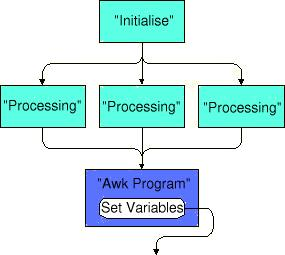
\includegraphics[width=7.459cm,height=6.747cm]{img/diag2.jpg}
\end{figure}
An \progname{awk} program could parse the output of the preceding jobs, executing the \PrBtvar{} command to set any number of
variables, affecting how the rest of the schedule will run.

Alternatively the \progname{awk} program could be an exception handler, which analyses and corrects problems then restarts
the schedule.

\bigskip

\subsection{SQL}
Any Database Product which has a command interpreter that will take commands on standard input can be used in exactly the same way as the
\progname{awk} example. This would be good for people writing SQL, on PCs for example, who do not have an Unix experience.

\subsection{A dummy Shell}
A command interpreter could be written to bypass or dummy\_run jobs, by reading the job but not executing any of the commands. To \ProductName{} it as though the job ran and finished normally. This could be used for testing schedules of jobs without doing any processing.

A shell script for such a command interpreter might look like this:

\begin{expara}

\#!/bin/sh

echo Job bypassed

exit 0

\end{expara}

The script could be expanded to check for job control variable operations that could invalidate testing a job schedule in this manner.

Another version could be set up that always exits with an error code. This command interpreter would be specified to simulate a job running
and failing.

\section{Scripts \& Macros}
The command line programs for \ProductName{} enable all job, variable, user and general information to be queried and/or modified. These can be built into new commands using shell scripts or used within user applications and used as macros.

This section gives some more ideas:

\subsection{Changing several Job Parameters in One Operation}
If a number of job parameters are often set to the same value, a macro can be created to apply this specification. For example: A particular type of job may be submitted for testing and when satisfactory changed over to production. The parameters to change for production work are:

\hspace{2cm}
\begin{tabular}{l l}
Time and Repetition & Run every day after 18:30\\
Command Interpreter & Change from sh\_debug to sh.\\
Queue name & Same as for testing but prefixed with string P\_\\
\end{tabular}

A suitable shell script for setting up as a macro would use \PrBtjlist{} to get the current queue name and
\PrBtjchange{} to apply the changes. It is as simple as this:

\begin{expara}

QNAME={\textasciigrave}\BtjlistName{} -F {\textquotedbl}\%q{\textquotedbl} \$1{\textasciigrave}

\BtjchangeName{} -T 18:30 -r Days:1 -q P\_\$\{QNAME\} -i sh \$1

\end{expara}

\PrBtq{} macro commands pass the currently-selected job number to the macro script.

The \PrBtjlist{} command could apply the prefix to the queue name like this:

\begin{expara}

QNAME={\textasciigrave}\BtjlistName{} -F {\textquotedbl}\textbf{P\_}\%q{\textquotedbl} \$1{\textasciigrave}

\BtjlistName{} -T 18:30 -r Days:1 -q \$QNAME -i sh \$1

\end{expara}

In practice several standard configurations are likely to be required. Rather than use a separate macro for each, the macro could be enhanced to give a list of suitable specifications for the job and ask the user to select one.

\subsection{Customising an Existing Command}
The built in delete command does not do anything about output files produced by jobs. Here is a shell script which deletes the job, then
any files produced for standard out and standard error:

\begin{exparasmall}

\#!/bin/ksh

\# Get the list of I/O redirections for the job. Separate each

\# redirection out - one per line. Substitute the job id for

\# any \%d1 in path/file names. Put results in a temporary file

\bigskip

TEMP=/tmp/jobredirs\$\$

\bigskip

\BtjlistName{} -F {\textquotedbl}\%R{\textquotedbl} \$1 {\textbar} sed -e
{\textquotedbl}s/\%d1/\$1/g{\textquotedbl} -e
{\textquotedbl}s/{\textgreater}{\textgreater}/{\textgreater}/g{\textquotedbl}
{\textbar}{\textbackslash}

awk -F, {\textquotesingle}\{ for ( i = NF; i {\textgreater}= 1; i-{}- )
print \$i \}{\textquotesingle} {\textgreater} \$TEMP

\bigskip

\# cd to the working directory for the job, to cope with

\# relative path names for output files.

\bigskip

cd {\textasciigrave}\BtjlistName{} -F {\textquotedbl}\%D{\textquotedbl}
\$1{\textasciigrave}

\bigskip

\# Attempt to delete the job, and abort if it is running.

\bigskip

\BtjdelName{} \$1

\bigskip

if [ ! -z {\textasciigrave}\BtjlistName{} -F {\textquotedbl}\%N{\textquotedbl}
\$1{\textasciigrave} ]

then

\ \ \ \ rm \$TEMP

\ \ \ exit 1

fi

\bigskip

\# Get the standard output and error file names.

\bigskip

OUTFILE={\textasciigrave}awk
-F{\textquotedbl}{\textgreater}{\textquotedbl} {\textquotesingle} \$1
!= 2 \&\& \$1 != 0 \{ print \$NF \}{\textquotesingle} \$TEMP
{\textasciigrave}

ERRFILE={\textasciigrave}awk
-F{\textquotedbl}{\textgreater}{\textquotedbl} {\textquotesingle}
/\^{}2/ \{ print \$NF \}{\textquotesingle} \$TEMP {\textasciigrave}

\bigskip

\# If the files exist then delete them. Then tidy up.

\bigskip

if [ ! -z {\textquotedbl}\$OUTFILE{\textquotedbl} ]

then if [ -f {\textquotedbl}\$OUTFILE{\textquotedbl} ]

\ \ \ \ \ then rm \$\{OUTFILE\}

\ \ \ \ fi

fi

\bigskip

if [ ! -z {\textquotedbl}\$ERRFILE{\textquotedbl} ]

then if [ -f {\textquotedbl}\$ERRFILE{\textquotedbl} ]

\ \ \ \ \ then rm \$\{ERRFILE\}

\ \ \ \ \ fi

fi

\bigskip

rm \$TEMP

exit 0

\end{exparasmall}

This example was built and tested on a Sun running Solaris with the version of \progname{awk} supplied as standard. If your
version of \progname{awk} does not work check the pattern syntax.

To implement the script as a macro:

\begin{itemize}
\item Disable the standard delete command by commenting out the key definition:

\begin{expara}

\# 1K501:D

\end{expara}

\item Specify the path and name of the shell script to be run. If the script is defined as the first macro this might look like:

\begin{expara}

27100P:/usr/macros/deljob

\end{expara}

\item Finally set up the macro key definition using the same key as the original delete command. For the first macro this will be:

\begin{expara}

1K701:D

\end{expara}
\end{itemize}

